% Gemini theme
% https://github.com/anishathalye/gemini
%
% We try to keep this Overleaf template in sync with the canonical source on
% GitHub, but it's recommended that you obtain the template directly from
% GitHub to ensure that you are using the latest version.

\documentclass[final]{beamer}

% ====================
% Packages
% ====================


\newcommand{\off}{\operatorname{off}}
\newcommand{\on}{\operatorname{on}}
\newcommand{\gX}{\mathcal{X}}
\newcommand{\gA}{\mathcal{A}}
\newcommand{\gS}{\mathcal{S}}
\newcommand{\gF}{\mathcal{F}}
\newcommand{\gT}{\mathcal{T}}
\newcommand{\gL}{\mathcal{L}}
\newcommand{\Reg}{\text{Reg}}
\usepackage[T1]{fontenc}
%\renewcommand{\thefootnote}{\arabic{footnote}}
\usepackage{boldline}
\usepackage{color}
%\usepackage[symbol]{footmisc}
\usepackage{lmodern}
\usepackage[size=custom,width=36,height=24,scale=1]{beamerposter}
\usetheme{gemini}
\usecolortheme{gemini}
\usepackage{natbib}
\usepackage{graphicx}
\usepackage{booktabs}
\usepackage{tikz}
\usepackage{pgfplots}
\usepackage{verbatim}
%%%%% NEW MATH DEFINITIONS %%%%%
\usepackage{amsmath,bbm,bm}
\usepackage{amssymb}
\usepackage{amsfonts}
\usepackage{amsthm}
\usepackage{mathtools}

% commands
% global count (no section number)
\newtheorem{thm}{Theorem}%[section]
\newtheorem{lem}{Lemma}
\newtheorem{prop}{Proposition}
\newtheorem{cor}{Corollary}
\newtheorem{conj}{Conjecture}
\newtheorem{aspt}{Assumption}
\newtheorem{claim}{Claim}
\newtheorem{rmk}{Remark}
\newtheorem{commt}{Comment}
\newtheorem{defn}{Definition}

% algorithm
%\usepackage{algorithm, algorithmic}
%\usepackage{algorithm2e}
\usepackage{tabularx}
%\usepackage[table,xcdraw]{xcolor}

% Comments
% \usepackage{xcolor} % already loaded
\newcount\comments  % 0 suppresses notes to selves in text
\comments=1  % TODO: change to 0 for final version
\newcommand{\genComment}[2]{\ifnum\comments=1{\textcolor{#1}{\textsf{\footnotesize #2}}}\fi}
\newcommand{\ed}[1]{\genComment{red}{[EI:#1]}}
\newcommand{\giles}[1]{\genComment{green}{[GH:#1]}}
\newcommand{\kevin}[1]{\genComment{blue}{[KT:#1]}}


% Mark sections of captions for referring to divisions of figures
\newcommand{\figleft}{{\em (Left)}}
\newcommand{\figcenter}{{\em (Center)}}
\newcommand{\figright}{{\em (Right)}}
\newcommand{\figtop}{{\em (Top)}}
\newcommand{\figbottom}{{\em (Bottom)}}
\newcommand{\captiona}{{\em (a)}}
\newcommand{\captionb}{{\em (b)}}
\newcommand{\captionc}{{\em (c)}}
\newcommand{\captiond}{{\em (d)}}


\newcommand\seq[2]{{#1}\!:\!{#2}}
\newcommand\R{\mathbb{R}}
\newcommand\Var{\mathrm{Var}}
\newcommand\var{\Var}
\newcommand\Cov{\mathrm{Cov}}
\newcommand\cov{\Cov}
\newcommand\iid{\mathrm{iid}}
\newcommand\dist{d}
\newcommand\lik{\mathcal{L}}
\newcommand\prob{\mathbb{P}}
\newcommand\E{\mathbb{E}}
\newcommand\loglik{\ell}
\newcommand\process{\texttt{process}}
\newcommand\dimtheta{\mathrm{dim}_{\Theta}}
\newcommand\param{\,;}
\newcommand\giventh\param
\newcommand\given{{\,\vert\,}}
\newcommand\code[1]{\texttt{#1}}
\newcommand\ceil[1]{\lceil #1 \rceil}
\newcommand\floor[1]{\lfloor #1 \rfloor}
\newcommand\1{\bm{1}}


% Highlight a newly defined term
\newcommand{\newterm}[1]{{\bf #1}}


% Figure reference, lower-case.
\def\figref#1{figure~\ref{#1}}
% Figure reference, capital. For start of sentence
\def\Figref#1{Figure~\ref{#1}}
\def\twofigref#1#2{figures \ref{#1} and \ref{#2}}
\def\quadfigref#1#2#3#4{figures \ref{#1}, \ref{#2}, \ref{#3} and \ref{#4}}
% Section reference, lower-case.
\def\secref#1{section~\ref{#1}}
% Section reference, capital.
\def\Secref#1{Section~\ref{#1}}
% Reference to two sections.
\def\twosecrefs#1#2{sections \ref{#1} and \ref{#2}}
% Reference to three sections.
\def\secrefs#1#2#3{sections \ref{#1}, \ref{#2} and \ref{#3}}
% Reference to an equation, lower-case.
\def\eqref#1{equation~\ref{#1}}
% Reference to an equation, upper case
\def\Eqref#1{Equation~\ref{#1}}
% A raw reference to an equation---avoid using if possible
\def\plaineqref#1{\ref{#1}}
% Reference to a chapter, lower-case.
\def\chapref#1{chapter~\ref{#1}}
% Reference to an equation, upper case.
\def\Chapref#1{Chapter~\ref{#1}}
% Reference to a range of chapters
\def\rangechapref#1#2{chapters\ref{#1}--\ref{#2}}
% % Reference to an algorithm, lower-case.
% \def\algref#1{algorithm~\ref{#1}}
% % Reference to an algorithm, upper case.
% \def\Algref#1{Algorithm~\ref{#1}}
% \def\twoalgref#1#2{algorithms \ref{#1} and \ref{#2}}
% \def\Twoalgref#1#2{Algorithms \ref{#1} and \ref{#2}}
% Reference to a part, lower case
\def\partref#1{part~\ref{#1}}
% Reference to a part, upper case
\def\Partref#1{Part~\ref{#1}}
\def\twopartref#1#2{parts \ref{#1} and \ref{#2}}

\def\eps{{\epsilon}}

\def\gN{{\mathcal{N}}}
\def\gX{{\mathcal{X}}}
\def\gY{{\mathcal{Y}}}


\makeatletter
\newcommand*{\addFileDependency}[1]{% argument=file name and extension
\typeout{(#1)}% latexmk will find this if $recorder=0
% however, in that case, it will ignore #1 if it is a .aux or 
% .pdf file etc and it exists! If it doesn't exist, it will appear 
% in the list of dependents regardless)
%
% Write the following if you want it to appear in \listfiles 
% --- although not really necessary and latexmk doesn't use this
%
\@addtofilelist{#1}
%
% latexmk will find this message if #1 doesn't exist (yet)
\IfFileExists{#1}{}{\typeout{No file #1.}}
}\makeatother

\newcommand*{\myexternaldocument}[1]{%
\externaldocument{#1}%
\addFileDependency{#1.tex}%
\addFileDependency{#1.aux}%
}
%\usepackage{enumitem}

\usepackage[skins,theorems]{tcolorbox}
%\tcbset{colback=white}

\definecolor{ballblue}{rgb}{0.13, 0.67, 0.8}
\definecolor{darkred}{RGB}{139,0,0}

\tcbset{highlight math style={enhanced,colframe=red,colback=white}}

\usepackage{colortbl} % Add this package to use \cellcolor
\definecolor{lightgreen}{rgb}{0.9, 1, 0.9} % Light green color definition


\pgfplotsset{compat=1.14}

% ====================
% Lengths
% ====================

% If you have N columns, choose \sepwidth and \colwidth such that
% (N+1)*\sepwidth + N*\colwidth = \paperwidth

\setlength{\paperwidth}{36in}
\setlength{\paperheight}{24in}


\newlength{\sepwidth}
\newlength{\colwidth}
\setlength{\sepwidth}{0.025\paperwidth}
\setlength{\colwidth}{0.3\paperwidth}

\newcommand{\separatorcolumn}{\begin{column}{\sepwidth}\end{column}}

\newcommand{\cross}[1][1pt]{\ooalign{%
  \rule[1ex]{1ex}{#1}\cr% Horizontal bar
  \hss\rule{#1}{.7em}\hss\cr}}% Vertical bar

% ====================
% Title
% ====================

\title{Automatic differentiation accelerates inference
for partially-observed Markov processes}

\author{Kevin Tan \inst{*} \and Giles Hooker \inst{*} \and Edward L. Ionides \inst{\cross[.4pt]$\cdot$}}

\institute[shortinst]{\inst{*} Department of Statistics and Data Science, University of Pennsylvania \quad  \inst{\cross[.4pt]} Department of Statistics, University of Michigan}

% ====================
% Footer (optional)
% ====================

\footercontent{
  \hfill
   \hfill
  }
% (can be left out to remove footer)

% ====================
% Logo (optional)
% ====================

% use this to include logos on the left and/or right side of the header:
 %\logoright{\includegraphics[scale=0.24]{logo1.png}}
%\logoleft{\includegraphics[scale=2.5]{sci logo.png}}

% ====================
% Body
% ====================

\begin{document}

\begin{frame}[t]
\begin{columns}[t]
\separatorcolumn

\begin{column}{\colwidth}

  \begin{block}{Introduction}
  
\textbf{Inference for continuous-time, continuous-state hidden Markov models.}

\begin{tcolorbox}[enhanced,colback=white!100!white,colframe=red!100!red]
\textbf{\textcolor{red}{Partially-Observed Markov Process}}: 

Unknown Markov process $(X_t)$, observations $y_1^*,...,y_N^*$ at $t_1,..., t_N$. \\
Estimate latent state of the system $x_{1:N}$ and system parameters $\theta \in \Theta$. 
\end{tcolorbox}
\small{e.g. given monthly cholera case counts, estimate number of infected and recovered people in the population, and how transmissible the disease is.}
  \end{block}


  \begin{block}{Problem}
  \vspace{-1.6ex}
  \begin{tcolorbox}[enhanced,colback=white!100!white,colframe=red!100!red]
  \begin{center}
  Maximum likelihood with only a simulator, cannot evaluate $f_{X_n|X_{n-1};\theta}$. \textbf{Cannot use the EM algorithm!}
  \end{center}
\end{tcolorbox}

  \textbf{What to do now?} Particle filters give a Monte Carlo approximation of the \textbf{filtering distribution} $f_{X_n|Y_{1:n};\theta}$ and the \textbf{log-likelihood} $\ell(\theta)$ increasingly accurate in the number of particles $J$. 
  %\vspace{1ex}
  
  \textbf{Idea:} Gradient descent using autodiff (AD) on the likelihood estimate? \textcolor{red}{But:}
  \vspace{-2.6ex}
  \begin{enumerate}
      \item Likelihood estimate not differentiable due to Monte Carlo resampling.
      \item Previous work \cite{corenflos21, naesseth18, poyiadjis11, scibior21} on this is computationally expensive \cite{corenflos21}, has uncontrolled asymptotic bias \cite{naesseth18}, or has high variance \cite{poyiadjis11, scibior21}. 
  \end{enumerate}
  \vspace{1ex}
  \end{block}
  
  \begin{alertblock}{Solution: Off-Parameter Resampling}

    \textbf{Reconstruct likelihood} at $\theta$ by cumulatively reweighting particles resampled at a \textbf{baseline parameter} $\phi \in \Theta$. Take gradient at $\theta=\phi$.

    \textbf{Smooth approximation:} Treating the particles at $\phi$ as constants, this is a function of a differentiable simulator and measurement density ratios, so the resulting likelihood estimate is smooth!

    \textbf{Bias-variance tradeoff:} Discount cumulative reweighting by $\alpha \in [0,1]$.

  \end{alertblock}

  \vspace{1ex}
    \begin{figure}
        \centering
        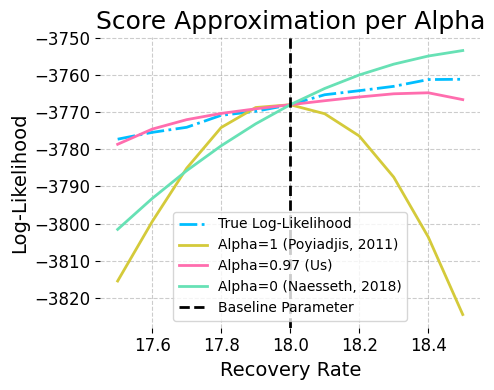
\includegraphics[width=0.52\linewidth]{imgs/095/mop.png}
        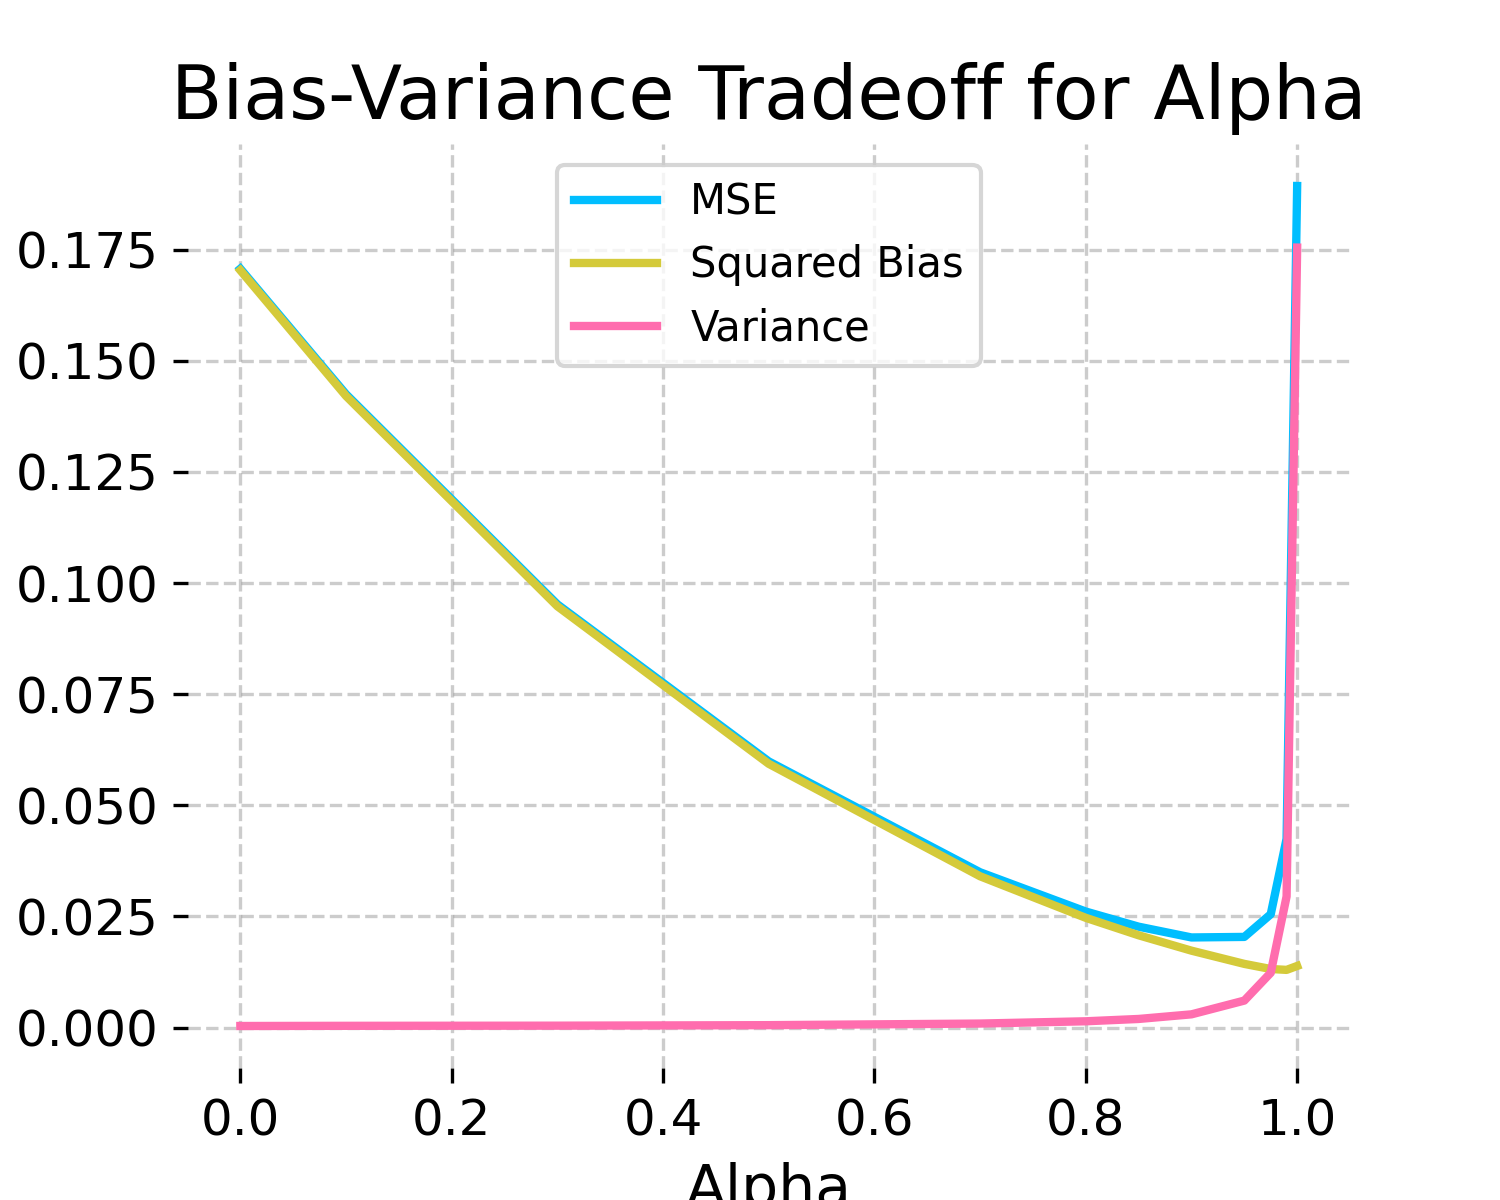
\includegraphics[width=0.472\linewidth]{imgs/095/biasvar.png}
        \caption{\textbf{Left:} Non-differentiable likelihood estimates and our smooth off-parameter reconstructions. 
        \textbf{Right:} Bias-variance tradeoff in score estimation induced by $\alpha$.}
        \label{fig:enter-label}
    \end{figure}
    
%Only simulation-based method for maximum likelihood available \cite{ionides15} gets close (\~40 nats) to the MLE quickly, but fails to find it ($\geq 7$ nats away). 

% \vspace{0.5em}
%  \begin{alertblock}{tl;dr}
    
%     \begin{itemize}
%         \item Modified an optimistic algorithm for general function approximation algorithm called GOLF \cite{jin2021bellmaneluder, xie2022policy}. 
%         \item Including the offline dataset in parameter estimation achieves provable improvements in regret over pure offline/online learning. 
%         \vspace{0.5ex}
%         \item How? Consider {\it arbitrary} (not necessarily disjoint) partitions of the state-action space $\gX_{\off} \cup \gX_{\on} = \gX$.
%         \begin{itemize}
%             \item Bound regret by the coverage of the behavior policy on $\gX_{\off}$  and a complexity measure for online learning on $\gX_{\on}$.
%             \item Overall regret is characterized by the regret bound on the best possible partition -- even if the algorithm is unaware of it. 
%         \end{itemize}
%         \item Not specific to DISC-GOLF! Yields a general recipe for initializing generic online RL algorithms with offline data without full coverage.
%     \end{itemize}

%   \end{alertblock}

\end{column}


\separatorcolumn

\begin{column}{\colwidth}

  \begin{alertblock}{Guarantees}
    \begin{enumerate}
        \item \textbf{Correctness:} Procedure targets the filtering distribution $\pi_n(\theta)$, and is strongly consistent for the likelihood under $\theta$.\footnotemark[1]\footnotetext{\tiny{1. We also showed a more general result holds, that of a particle triangular array SLLN corrected for arbitrary off-target resampling.}}
        
        Obtains state estimates $x_{n,1:J}^{F,\theta}$ and a likelihood estimate $\hat \lik_J^\alpha(\theta)$ so for any $\alpha\in[0,1]$ and measurable bounded functional $h$, as $J \to \infty$:
        
  $$\frac{\sum_{j=1}^J h\left(x_{n, j}^{F, \theta}\right) w_{n, j}^{F, \theta}}{\sum_{j=1}^J w_{n, j}^{F, \theta}} \stackrel{\text{a.s.}}{\to} \E_{\pi_n(\theta)}[h(X_n)], \qquad \hat{\mathcal{L}}_J^\alpha(\theta) \stackrel{\text{a.s.}}{\to} \mathcal{L}(\theta).$$
  \vspace{1.5ex}
  
  \item \textbf{Consistent score estimates:} When $\alpha=1$, $$\nabla_\theta \hat\ell_J^1(\theta) \stackrel{\text{a.s.}}{\to} \ell(\theta) \text{ as } J \to \infty.$$ Else, increasing asymptotic bias as $\alpha \to 0$, but lower variance.
  \vspace{2ex}
  \item \textbf{Encompasses and interpolates between other estimators:}\\
  \textbf{$\alpha=0$:} $\nabla_\theta \hat\ell_J^0(\theta)$ is \cite{naesseth18}'s low-variance/asymptotically biased estimate. \\
  \textbf{$\alpha=1$:} $\nabla_\theta \hat\ell_J^1(\theta)$ is \cite{poyiadjis11}'s high-variance/consistent estimate.
  \vspace{2ex}
  \item \textbf{Linear convergence for gradient descent/quasi-Newton/Newton:} \\Early-stopped particle gradient descent with learning rate $\eta$, large $\alpha, J$ converges linearly if log-likelihood strongly convex and smooth:
  $$\ell\left(\theta^*\right)-\ell\left(\theta_{m+1}\right) \leq\left(1- O(\eta)\right)\left(\ell\left(\theta^*\right)-\ell\left(\theta_m\right)\right).$$
    \end{enumerate}
  \end{alertblock}

  %\vspace{-2.5ex}
  \begin{block}{Rates for Score Estimates}
  \vspace{-1.5ex}
      \begin{table}[t]
\centering
\scalebox{1}{
\begin{tabular}{c  c}
\toprule \multicolumn{2}{c}{\textbf{MSE}} 
\tabularnewline
\toprule 
\vspace{1.2ex}
$\alpha \in (0,1)$ & \qquad$\tcbhighmath[colframe=ballblue]{\min_{k \leq N} N p (k^2/J+
\begingroup
\color{ballblue}\underbracket[1pt][1pt]{\color{black}
(1-\epsilon)^{\lfloor k /(c \log (J))\rfloor}}_{\text{\textcolor{blue}{\tiny{controllable bias}}}}
\endgroup
+k+\psi_k(\alpha))}$\qquad
\vspace{0.2ex}
\tabularnewline \hline
\vspace{0.2ex}
$\alpha=0$ \cite{naesseth18} & $N p (1/J + 
\begingroup
\color{red}\underbracket[1pt][1pt]{\color{black}(1-\epsilon)^{\lfloor 1 /(c \log (J))\rfloor}}_{\text{\textcolor{red}{\tiny{uncontrollable bias}}}}
\endgroup
)$
\vspace{0.2ex}
\tabularnewline
\hline
\vspace{0.2ex}
$\alpha=1$ \cite{poyiadjis11} & $N^4p/J$
\vspace{0.2ex}
\tabularnewline
\toprule
  \multicolumn{2}{c}{\textbf{Variance}}
\tabularnewline
\toprule\vspace{0.2ex}
$\alpha \in (0,1)$ & $\tcbhighmath[colframe=ballblue]{\min _{k \leq N}Np\left(\frac{k^2}{(1-\alpha)^2 J}+\frac{\alpha^k}{1-\alpha} \right)}$
\vspace{0.2ex}
\tabularnewline \hline
\vspace{0.2ex}
$\alpha=0$ \cite{naesseth18} & $N p /J$
\vspace{0.2ex}
\tabularnewline
\hline
\vspace{0.2ex}
$\alpha=1$ \cite{poyiadjis11} & $N^4p/J$
\vspace{0.2ex}
\tabularnewline
\toprule 
\end{tabular}}
\medskip
\caption{Rates given the trajectory length $N$, number of particles $J$, parameter space dimension $p$, model-specific constant $\epsilon>0$, where $\psi_k(\alpha)=\left(\alpha^k+\alpha^{k+1}-\alpha\right) /(1-\alpha)$. 
\textcolor{red}{Our $\alpha \in (0,1)$ has a better rate for the MSE than $\alpha=0$ \cite{naesseth18} and $\alpha=1$ \cite{poyiadjis11}.}}
\label{tab:bounds}
\vspace{-5mm}
\end{table}
  \end{block}

\end{column}

\separatorcolumn
\begin{column}{\colwidth}

\vspace{-2ex}
\begin{figure}[H]
    \centering{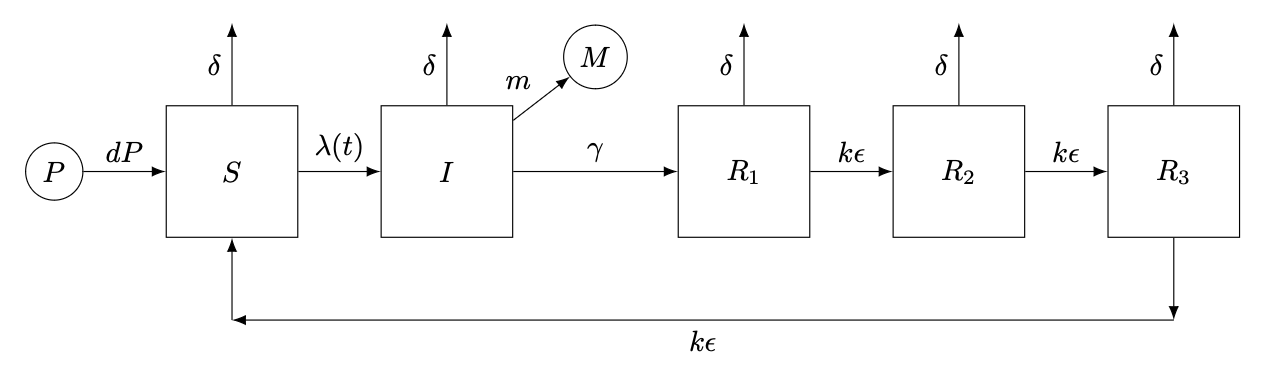
\includegraphics[scale=1]{imgs/095/tikzcholera.png}}
    \vspace{-2ex}
    \caption{Diagram of the stochastic SIRS model in \cite{king08}. 
    }
\end{figure}

\vspace{.5ex}
  \begin{exampleblock}{Case Study: Cholera Epidemic in Dhaka, Bangladesh}

  \textbf{Dhaka, 1821-1940:} Stochastic SIRS model from \cite{king08}. Cholera dynamics governed by SDEs. Seasonality, trend in infection modeled with splines.

  \textbf{In practice:} Gradient descent got stuck. Needed a warm-start with IF2 \cite{ionides15} to get to a neighborhood of the MLE quickly and find the MLE.
  \vspace{0.8ex}
  
    \begin{figure}[H]
    \centering
    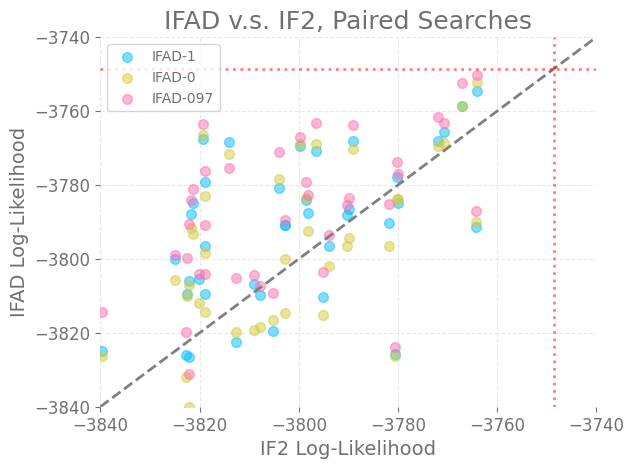
\includegraphics[scale=1.15]{imgs/095/pairs.png}
    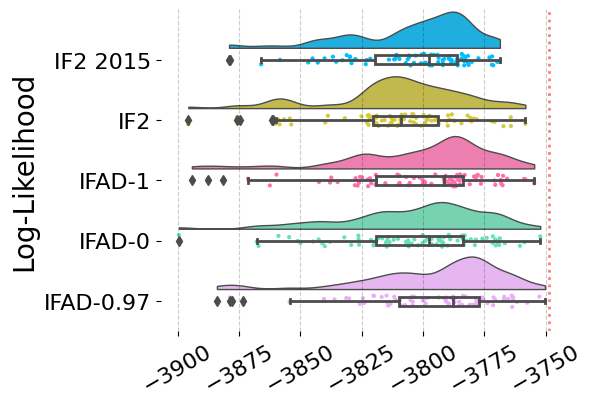
\includegraphics[scale=0.915]{imgs/095/boxplot_all.png}
    \caption{\textbf{Left:} Scatterplot depicting paired searches from the same starting point. \textbf{Right:} Raincloud plot of all searches. Our method outperforms the benchmark, IF2. }
    \label{fig:scatter-raincloud}
\end{figure}
%\vspace{1ex}

\begin{figure}[H]
    \centering
    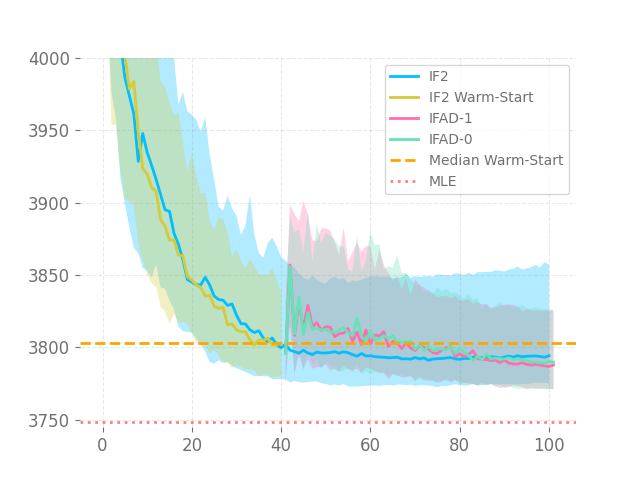
\includegraphics[scale=0.815]{imgs/095/optim.png}
    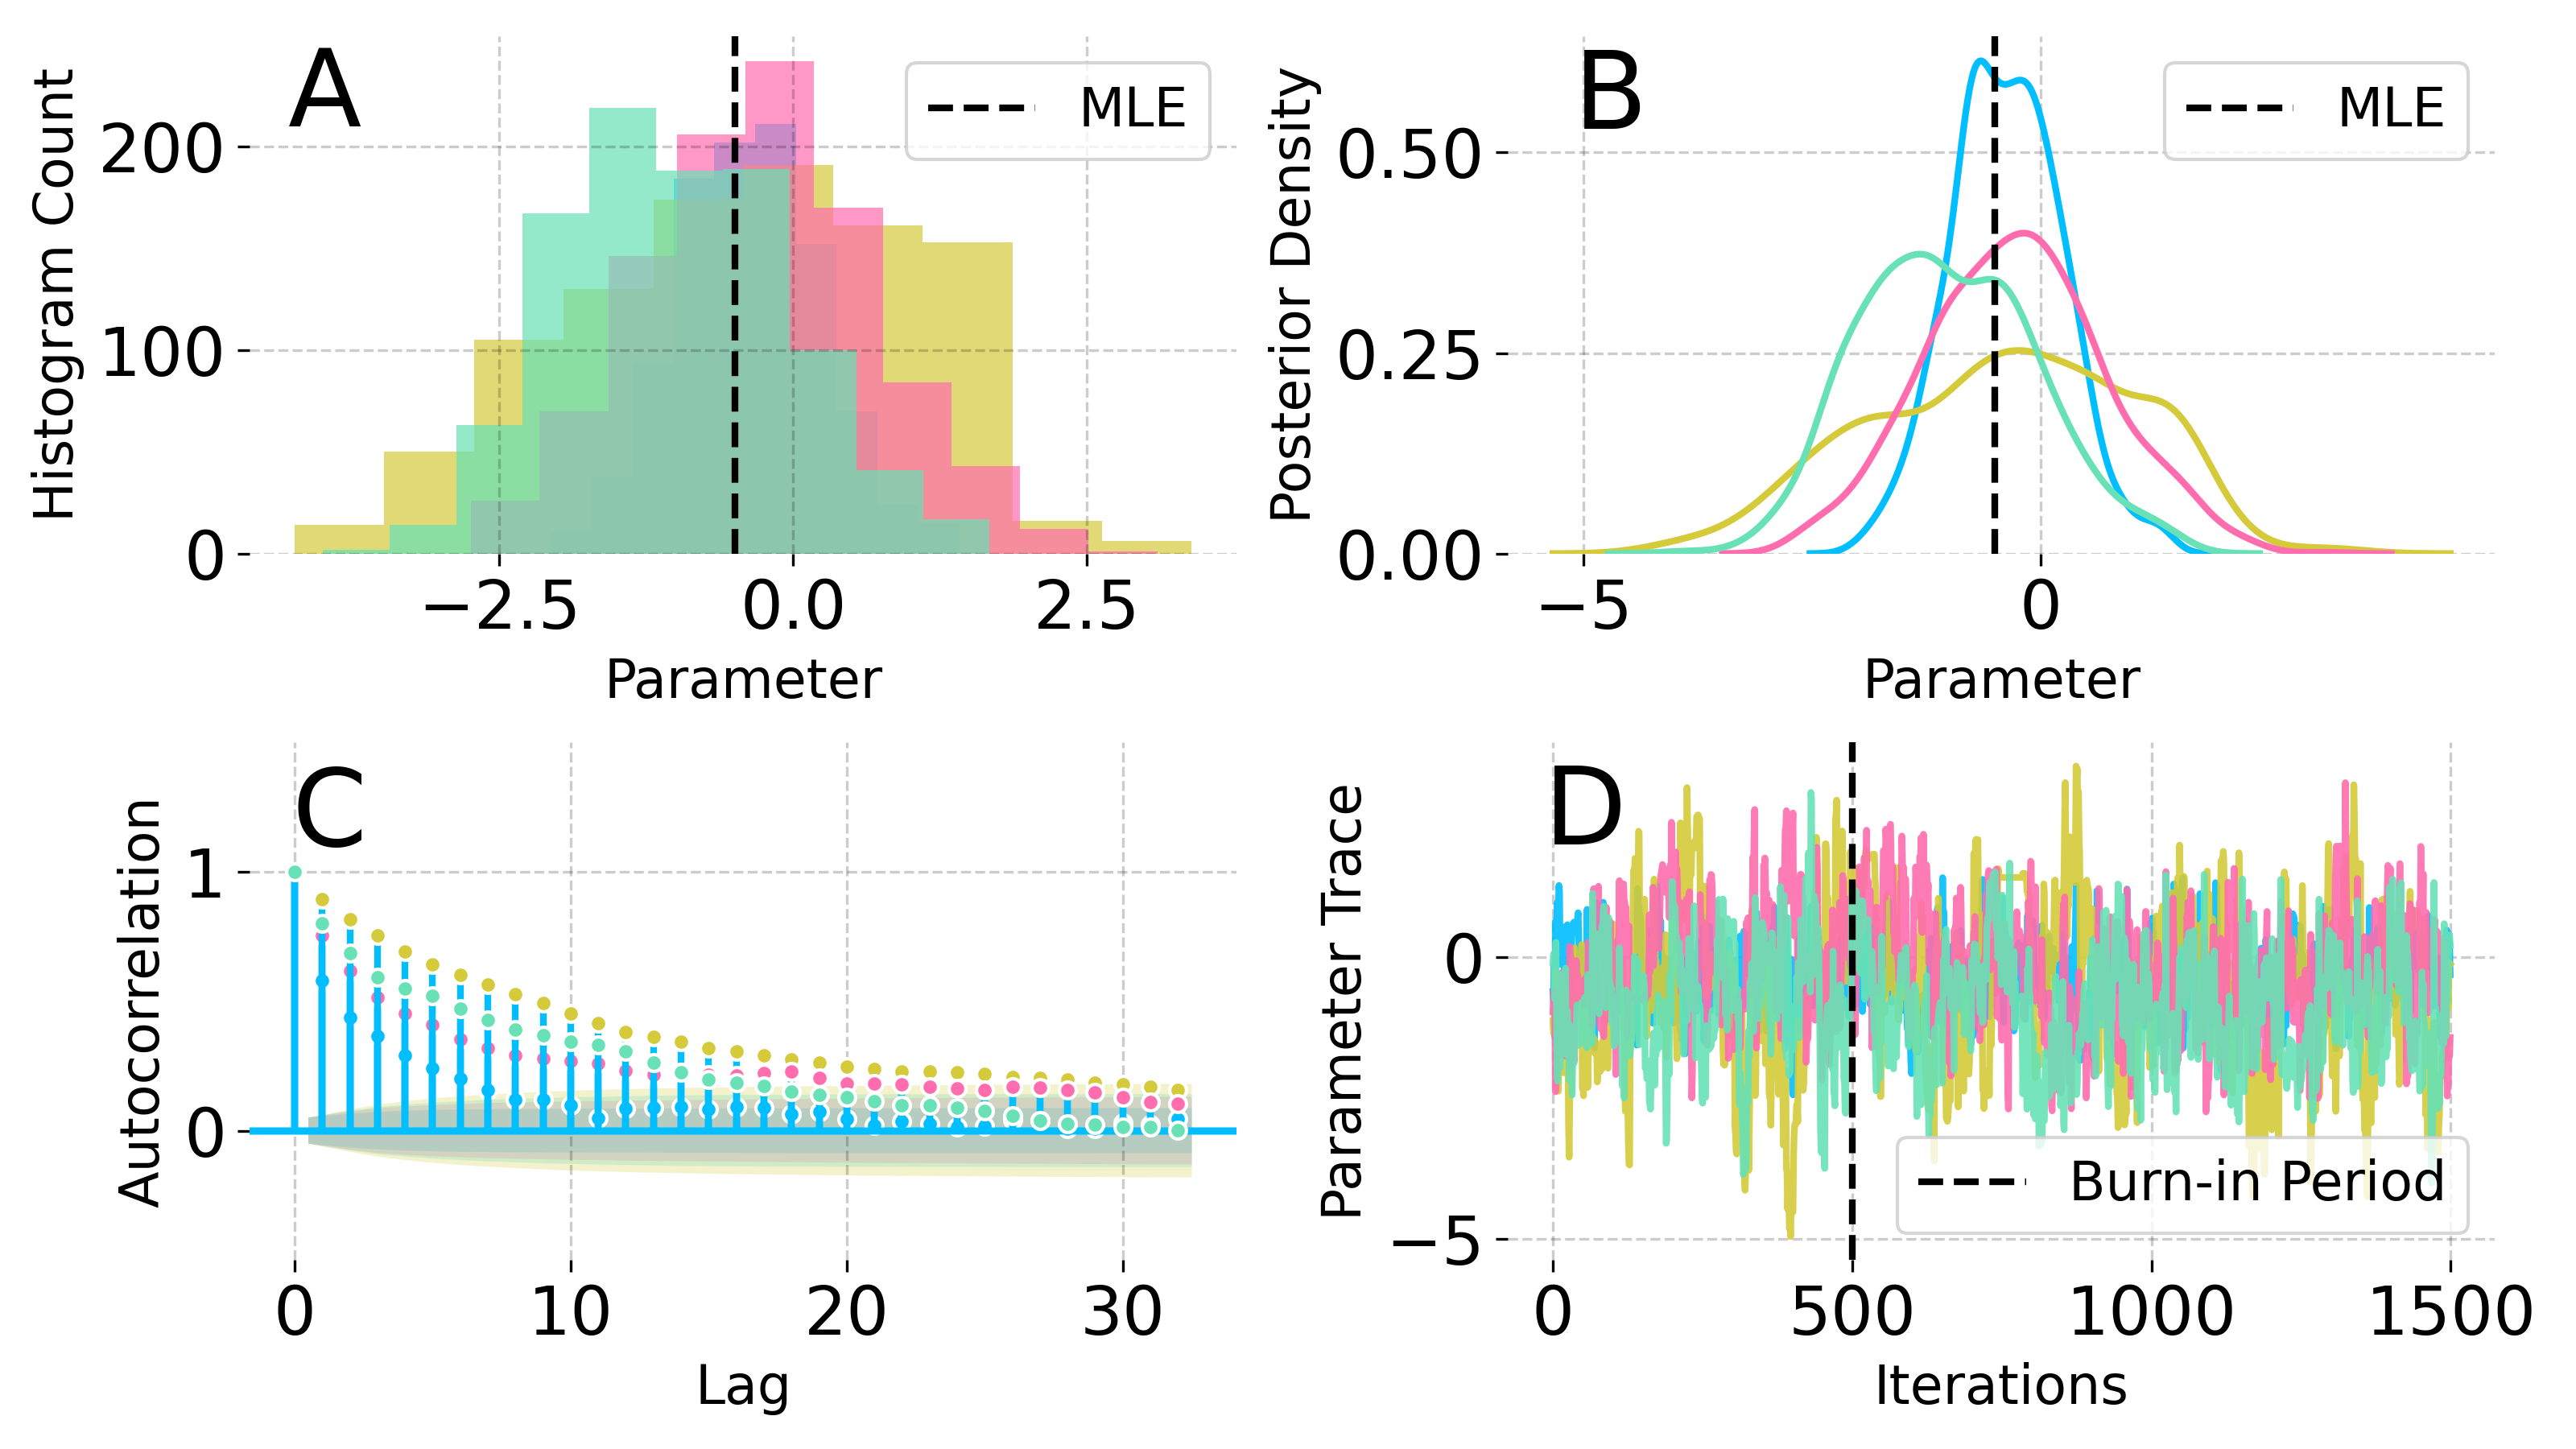
\includegraphics[scale=0.562]{imgs/pmcmc/nuts_eb.png}
    \caption{\textbf{Left:} Optimization progress of IFAD (ours) and IF2 \cite{ionides15} over 100 trials. \textbf{Right:} Application to Bayesian inference. 
    }
\end{figure}

    \textbf{Application to Bayesian inference:} Using our score estimate for a No U-Turn Sampler for particle MCMC, with an informative prior from the IF2 warm-start, reduces burn-in time from 700,000 \cite{fasiolo16} to 500 iterations.
  \end{exampleblock}


\vspace{-2ex}
  
%\vskip-1ex
\begin{block}{}
  \vspace{-0.5ex}
    \tiny{\bibliographystyle{plain}
    \bibliography{paper/bib-ifad}}
\end{block}



  %\vskip-1ex
  \vspace{0.2em}

  
  % \begin{block}{Contact Information}
  % \vskip-0ex
  %   %\nocite{*}
  %   \small{{Email Address}: kevtan@wharton.upenn.edu}
  % \end{block}

\end{column}

\separatorcolumn
\end{columns}
\end{frame}

\end{document}
